\documentclass[../report.tex]{subfiles}
\begin{document}
% Chapter State of the art
% - Concepts (before diving into the protocoles, it is important to understand some concepts)
% - Outlines of the KAPE landscape (all PAKEs, history, overview)
% - Mains PAKEs (differences, improvement, tableau comparatif, pas besoin de décrire les constructions)
%   - EKE
%   - SRP
%   - OPAQUE
%   - KHAPE
% - PAKE choice (and reasons)
% (Attack on PAKEs ?)

% Chapter OPAQUE or Chapter KHAPE (depending on the PAKE choice)
% - detail construction (protocol) of the choosen PAKE
\chapter{State of the art} \label{cha:state_of_the_art}
This chapter aims to provide a detailed view of the current PAKE landscape and its main protocols.
\section{Notation}
Schemas will use the notation described in Fig \ref{fig:notation}.
\begin{figure}[h]
 \centering
 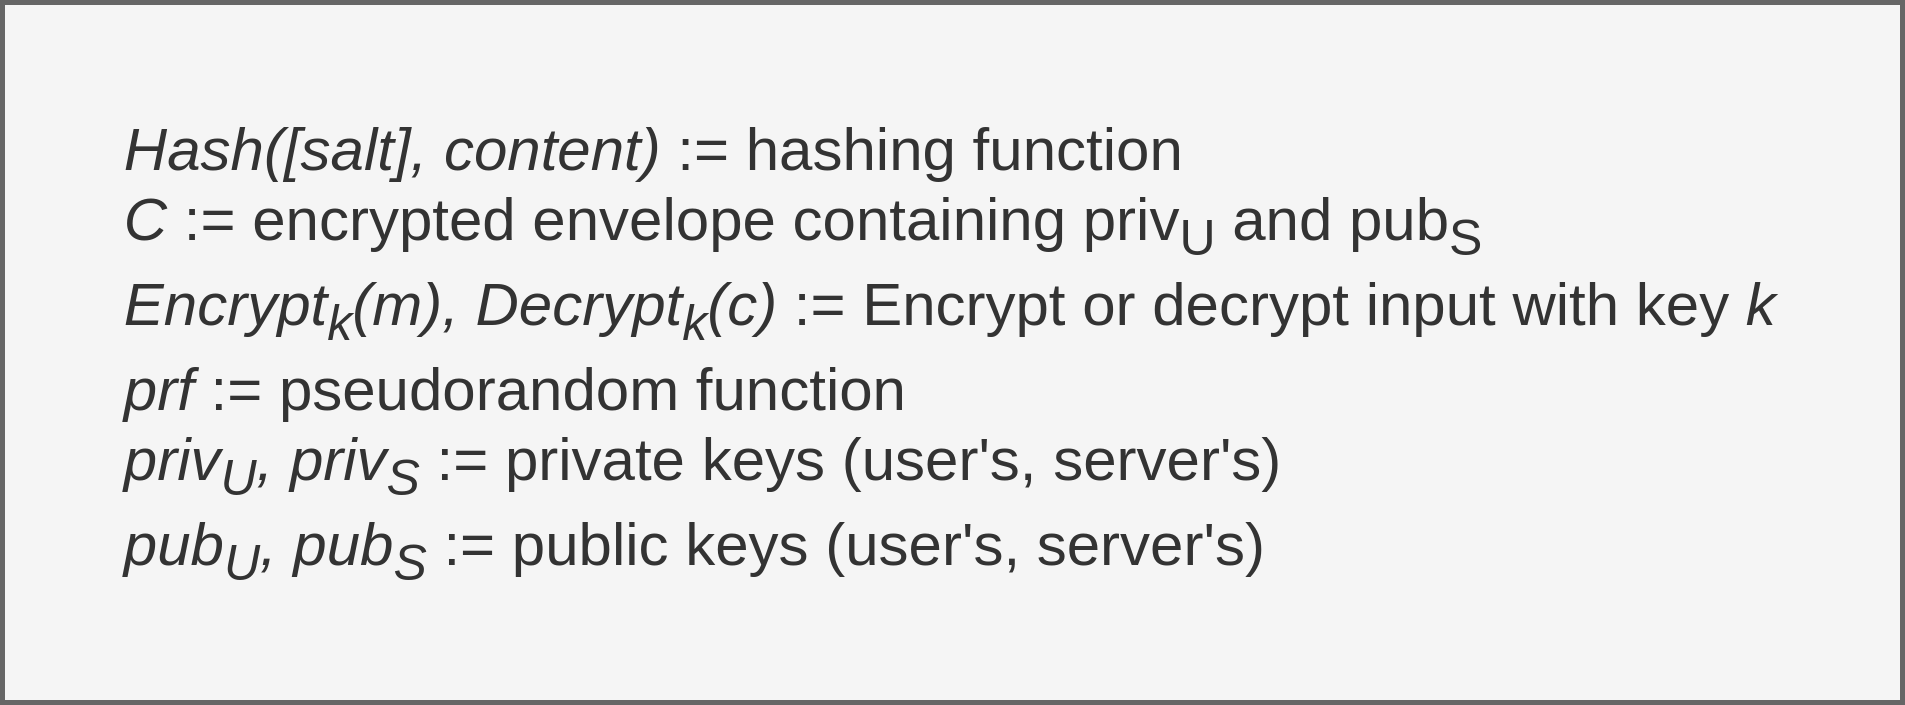
\includegraphics[width=10cm]{notation.png}
 \caption{Schema notation.}
 \label{fig:notation}
\end{figure}

% \section{History of PAKEs}
% citer, annee, artuble, ce qu0il fait, patent?, cassé ?, ce qu'il apport en plus, citer l'article et citer l'arcile qui l'a cassé. pourquoi il y a un saut entre SRP et OPAQUE (dans le temps) ?
% 
% \paragraph{EKE (1992).}
% Evolution and variants ?  in particular A-EKE which is the first aPAKE
% \paragraph{EKE variants (PAK, PPK, PAK-X).}
% \paragraph{OKE.}
% \paragraph{SNAPI.}
% \paragraph{PEKEP.}
% \subsection{Symmetric PAKE}
% \subsection{Asymmetric PAKE}
% \paragraph{SRP (1998).}
% \paragraph{OPAQUE (2018).}
% \paragraph{KHAPE (2021).}

\section{Main PAKEs}
This section describe in more details four fundamental PAKE construction. 
EKE as it is the first ever PAKE. 
SRP because it is the most used. 
OPAQUE because it is very promising, in the process of standardization and the first construction of this new generation of Strong aPAKE.
OPAQUE because it is the first construction of Strong aPAKE
KHAPE because it is most recent one and provide slightly better security guarantees than OPAQUE in certain conditions.

\subsection{\writingFormulationClean{EKE}}
\paragraph{\writingFormulationClean{Introduction.}}
EKE (for Encrypted Key Exchange) was proposed in 1992 by Bellovin and Merritt \cite{EKE_Paper} and is the first PAKE protocol. 
It allows two parties that share a common password to exchange information over an insecure channel.
It is a simple protocol that is designed to prevent offline dictionary attacks on the password.
It uses a combination of asymmetric and symmetric cryptography.
The asymmetric keys are ephemeral and are exchanged between the client and the server by encrypting it with the shared symmetric key --- which is derived from the password.
This allows securing the exchange against Man-in-the-middle attack. % more ?
It is a symmetric PAKE so it requires that both party share a secret --- namely the password. This means that the server has to store and process the password in cleartext which is strongly discouraged. % details ?

Multiple cryptographic primitive can be used for the asymmetric part such as RSA, ElGamal or DH but the majority of EKE variants use DH \cite{Breaking_EKE}. % more ? why ?
Note that some of the EKE variant got broken. 
% Some EKE variants got broken and therefore should not be used. % TODO source. all EKE ? DH-EKE also ? See http://www.jablon.org/jab96.pdf chapter 4
EKE was patented until 2011 which might have severely impacted its adoption.

% ``Diffie-Hellman Encrypted Key Exchange (DH-EKE) is the earliest widely deployed PAKE. It works by encrypting the public keys of a Diffie-Hellman key exchange with a shared secret. However, it requires both that unauthenticated encryption be used and that the public keys be indistinguishable from random data. This last requirement makes it impossible to use this form of PAKE with elliptic curve cryptography. For these reasons, DH-EKE is not a good fit.'' Source : https://tools.ietf.org/id/draft-ietf-kitten-krb-spake-preauth-00.html#rfc.section.1.2


\paragraph{\writingFormulationClean{Construction.}}

\begin{figure}[h]
 \centering
 \setlength{\fboxsep}{10pt}
 \setlength{\fboxrule}{1pt}
 \fbox{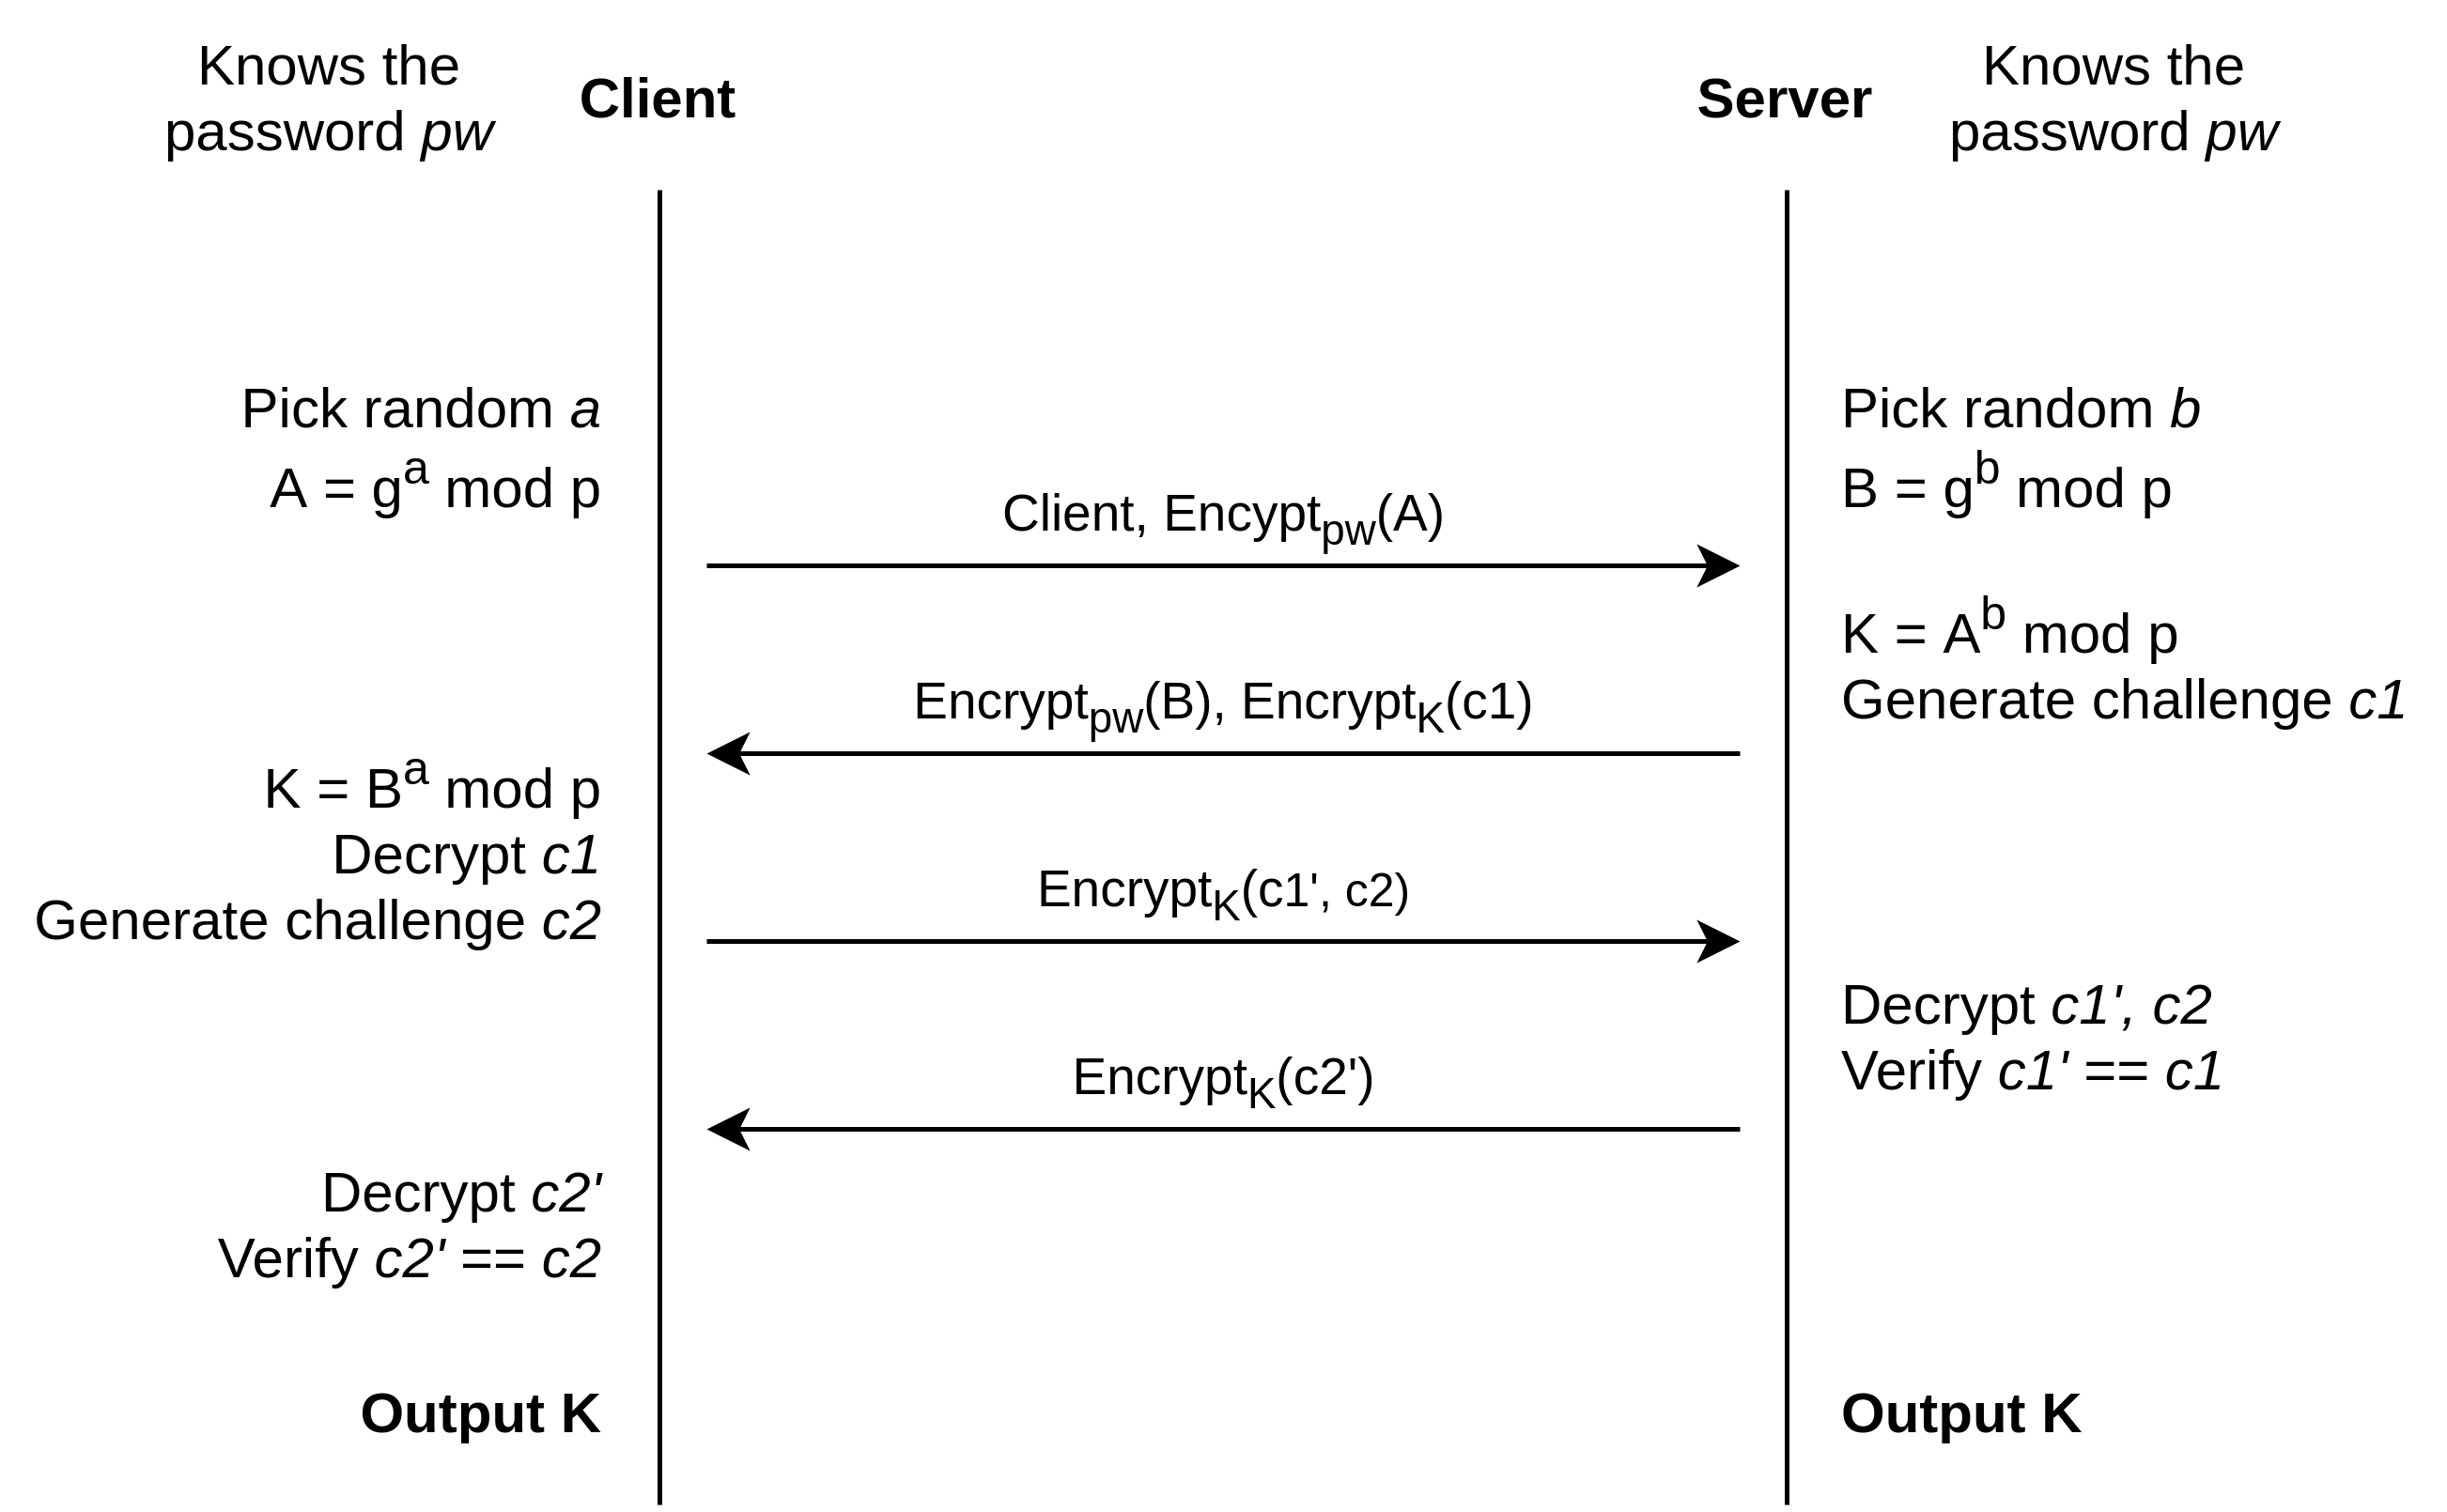
\includegraphics[width=\textwidth-22pt]{EKE.png}}
 \caption{Login process with EKE (DH-EKE) protocol.}
 \label{fig:EKE_DH}
\end{figure}
The figure \ref{fig:EKE_DH} shows the EKE protocol --- built with DH ---  during login process.
The steps are the following :
\begin{enumerate}
 \item Like a standard DH exchange, both client and server pick a random secret value $a$ and $b$.
 \item Client computes $A$, encrypt it using the password and send the result to the server in addition to it identifies (e.g., username).
 \item Server decrypts ciphertext using the password to obtain $A$. He computes $B$ and $K$. He encrypts $B$ using the password and encrypt a randomly generated challenge $c1$ using $K$. He sends the resulting ciphertext to the client.
 \item The client decrypts $B$ using the password and compute $K$. He decrypts $c1$ with $K$ and also generate a random challenge $c2$. He concatenate the two challenges, encrypt them using $K$ and send the result to the server.
 \item Server decrypt the ciphertext and check that both sent and received $c1$ match. If it is the case, the server is assured that the client possesses the same password. The server has authenticated the client. He finishes by encrypting $c2$ and sending the result.
 \item Client decrypts the ciphertext and check that both sent and received $c2$ match. If it is the case, the client is assured that the server possesses the same password and therefore is authenticated. The client has authenticated the server.
\end{enumerate}

%%% Login ?
\paragraph{\writingFormulationClean{Register.}}
The protocol does not mention registration. It is assumed that both parties already share a common secret, the password. A secure channel is therefore necessary to share the password in the first place.

% ====================================================================================

\subsection{\writingNotes{SRP}}
\paragraph{\writingNotes{Introduction.}}
SRP \cite{SRP_Paper, SRP_6_Paper} (for Secure Remote Password) was proposed in 1998 and is the most widely implemented PAKE protocol in the world \cite{PAKE_Green_blog}.
It is largely used in iCloud Key Vault --- which could make it one of the most widely used cryptographic protocols \cite{PAKE_Green_blog} considering the number of active Apple devices worldwide --- and in 1Password's password manager.
It is well standardized and has numerous implementation in different programming languages. %\cite{http://srp.stanford.edu/links.html}.
It is in fact a TLS cipher suite \cite{SRP_RFC_3}, implemented in OpenSSL.
This success is partly due to the SRP's creators will to avoid patents --- unlike most of the PAKE of its time --- but also to avoid export restriction imposed by US law by not using any encryption schema \cite{SRP_Formal_Analysis}.
Their goal was to provide a technology that improve the security of existing password protocols while keeping the ease-of-use of passwords. In other words, provide a drop-in replacement to the classical authentication methods where the implementation does not require a deep change in contrary to EKE where the shared secret --- the password --- need to be stored in cleartext on the server making it difficult to manage correctly.
This makes SRP easy to implement for developers and transparent for the user.
One of the main strengths of SRP is that the server does not store the cleartext password or the hashed password. Instead it stores a password verifier that is a discrete logarithm one-way function of the password.

Even though SRP is in interesting construction and does some things right, it is not ideal.
It got broken and patched multiple time --- current version is SRP v6a, which is not broken.
It is vulnerable to pre-computation attack because the server sends the cleartext salt to the client at the start of the exchange. With the salt, an adversary could build a table of password hashes --- a time-consuming process --- before compromising the server making it able to retrieve passwords instantaneously upon server compromise.
In addition, the construction is weirdly complex.
The protocol mix addition and multiplication in calculation. Using both operations require a ring rather than a cyclic group. This requirement makes it impossible to easily transfer the integer-based algorithm to elliptic curves. % because in integer-based group like DH, multiplication become EC point addition in ECC. SRP use both mutliplication and addition
This requirement, also makes it challenging to provide a formal analysis of SRP because 
``existing tools provide no simple way to reason about its use of the mathematical expression $v+g^b \mod{q}$'' \cite{SRP_Formal_Analysis}. % TODO rephraase and add this to comparison details

\paragraph{\writingFormulationClean{Construction.}}

\begin{figure}[h]
 \centering
 \setlength{\fboxsep}{10pt}
 \setlength{\fboxrule}{1pt}
 \fbox{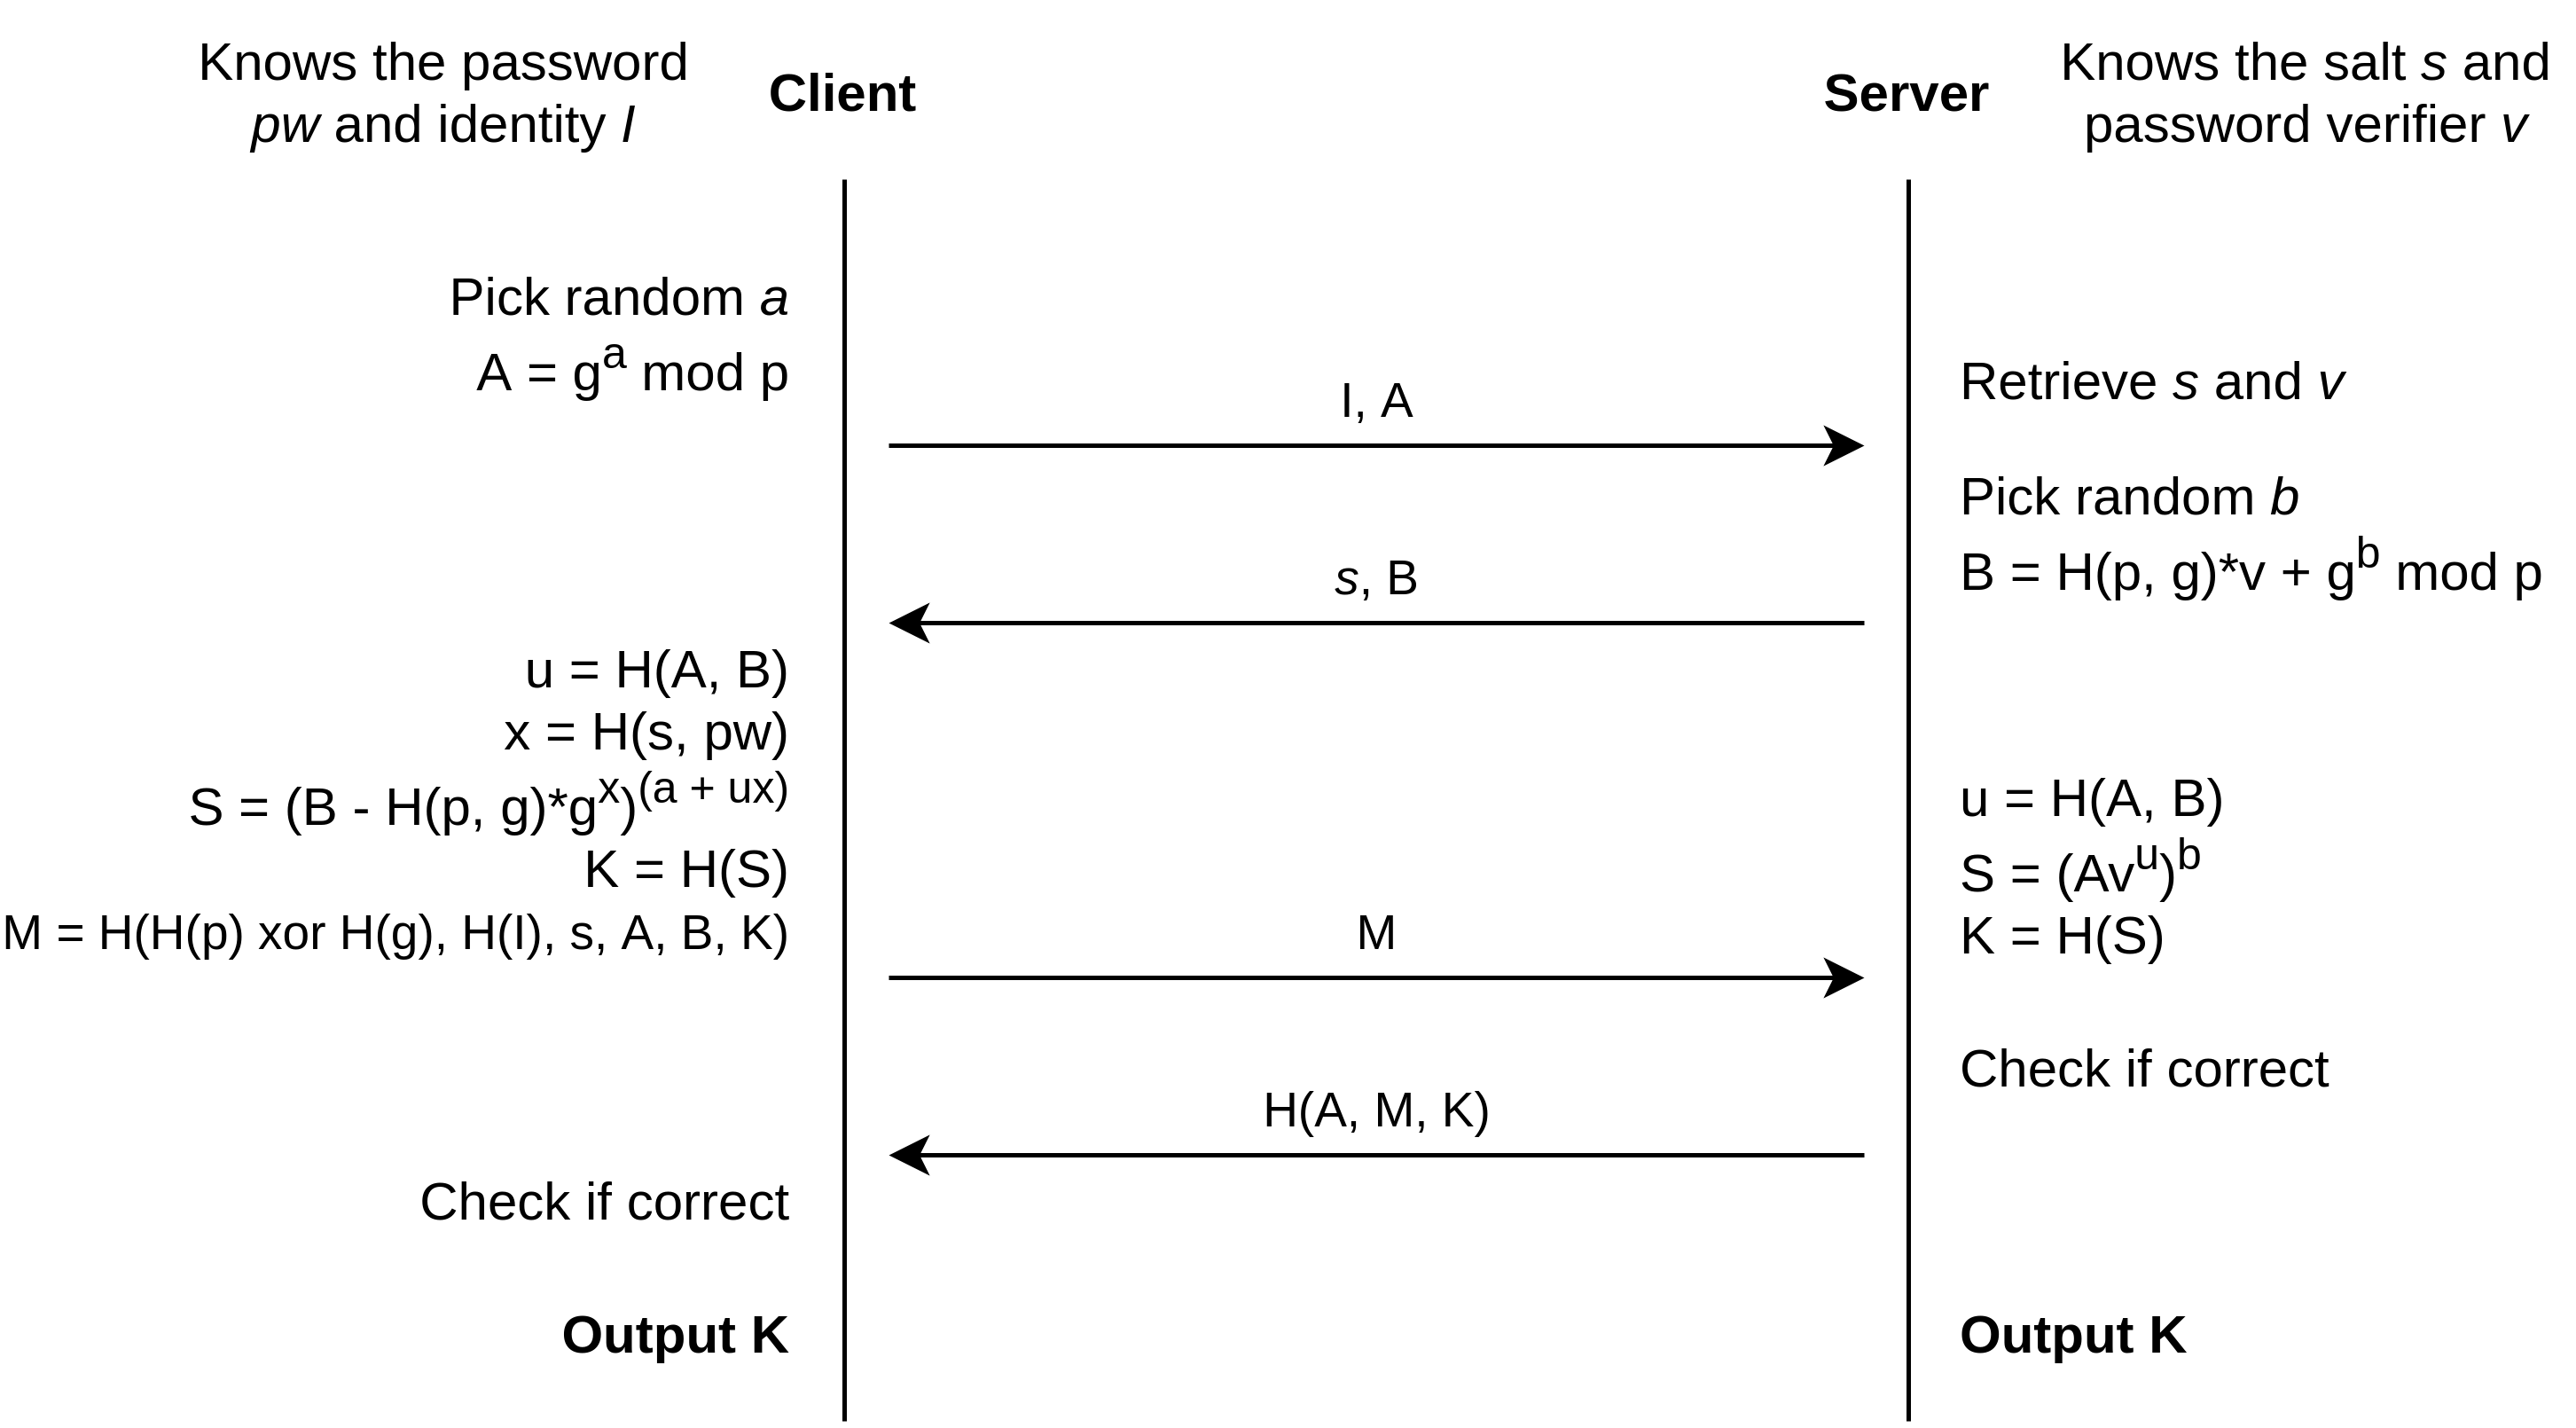
\includegraphics[width=\textwidth-22pt]{SRP.png}}
 \caption{Login process with SRP-6a protocol.}
 \label{fig:SRP}
\end{figure}
The figure \ref{fig:SRP} shows the SRP-6a protocol during login process.
The steps are the following :
\begin{enumerate}
 \item Client picks a random $a$ and computes $A$.
 \item The client sends $A$ and its identity $I$ (username) to the server.
 \item Server retrieves user salt $s$ and password verifier $v$ from its database using the user's identity.
 \item $v$ is computed at registration and is equal to $v = g^x$ where $x = H(s, pw)$
 \item Server also picks a random $b$ and computes $B$.
 \item The server sends $s$ and $B$ to the client.
 \item The client and server both compute $u$, $S$ and $K$ with their own values.
 \item They finish with a mutual key-confirmation process where the client sends his proof of $K$ first.
 \item If the server finds that the user's proof is incorrect, he stops the exchange and does not send its own proof of $K$.
\end{enumerate}
If the password is correct, the client and the server end up with having the same $S$ --- and so the same key. The derivation of $S$ is less straightforward than other constructions so it is detailed below.
\begin{align*}
 S_{client}
 &\equiv (B - H(p, g) g^x)^{(a+ux)}\notag\\
 &\equiv ((H(p, g) g^x + g^b) - H(p, g) g^x)^{(a+ux)}\notag\\
 &\equiv (g^b)^{a+ux}\notag\\
 &\equiv g^{ab+bux}\notag\\
 &\equiv (g^a (g^x)^u)^b\notag\\
 &\equiv (Av^u)^b\notag\\
 &\equiv S_{server} \pmod{p}
\end{align*}
\paragraph{\writingFormulationClean{Register.}}
The registration process is not covered in SRP papers.
Clients must come with a password, and server need to generate a random salt. One of them also need to compute the verifier $v = g^x$ where $x = H(salt, password)$.
This means that either the server sends the salt to the client and the client compute the verifier and send it back to the server through a secure channel (more secure as the server never see the user's password but more complicated to implement).
Or the client sends its password to the server with its registration request --- through a secure channel --- and the server generates a salt and computes the verifier (easier to implement on the server side, less transmission, but password is handled in cleartext on the server).
Either way, the registration require to use a secure channel.
Upon a successful registration, the server store the following triplet : \\
\verb|<username, verifier, salt>|


% ------------- Formal Methods Analysis of the Secure Remote Password Protocol (2020) -----------------
% "avoid export controls by not using encryption"
% "Formal analysis of SRP is challenging in part because existing tools provide no simple way to reason about its use of the mathematical expression   v+gbmodq ."

% ---------- SRP Stanford homepage -------------------
% - widly standaridized (3 RFC, IEEE, ISO ): http://srp.stanford.edu/doc.html#standards
% - SRP ciphersuite
% - multiple versions. SRP-3 (1998), evolved in SRP-6, now SRP-6a
% - no patent, royalty-free license, open source project. An exception because most of the PAKE in this time were patented (source ? CAA)
% - Adaptable to EC (NOT EASILY) : Y. K. Lee, J. K. Lee, "EC-SRP Protocol: Elliptic Curve Secure Remote Password Protocol", Korea Institute of Information Security and Cryptology, Vol 9, No. 1, pp. 85-102, 1999.
% - "SRP borrows some elements from other key-exchange and identification protcols and adds some subtle modifications and refinements. The result is a protocol that preserves the strength and efficiency of the EKE family protocols while fixing some of their shortcomings"
% - design of SRP-6 : http://srp.stanford.edu/design.html

%%% The Project 
% - "The primary goal of the SRP Project is to provide standards, technologies, and implementations that improve password security of existing protocols and applications while preserving the ease-of-use associated with passwords and integrating cleanly with these systems. SRP accomplishes these objectives because it was designed with a number of considerations in mind."
% - "SRP has been deployed as a secure, free password authentication solution in commercial, non-commercial, and standalone configurations in universities, companies, and organizations worldwide."
% - "SRP was designed to protect passwords against both passive and active network attacks"
% - "SRP has been extensively analyzed and studied in the open, and all analysis to date has confirmed its security"
% - "Convenience - From the perspective of some users, the fact that SRP keeps password interfaces exactly the same while delivering secure authentication is perhaps the greatest of its technical advances. Until now, users have had to compromise - either put up with some added inconvenience or accept an imperfect security model. SRP advances the status quo in both directions, achieving the best of both worlds in one package." Blackbox that doesn't require major interface changes.
% "Security, convenience, openness and simplicity"

%%% Abstract
% "This paper presents a new password authentication and key-exchange protocol suitable for authenticating users and exchanging keys over an untrusted network. The new protocol resists dictionary attacks mounted by either passive or active network intruders, allowing, in principle, even weak passphrases to be used safely. It also offers perfect forward secrecy, which protects past sessions and passwords against future compromises. Finally, user passwords are stored in a form that is not plaintext-equivalent to the password itself, so an attacker who captures the password database cannot use it directly to compromise security and gain immediate access to the host. This new protocol combines techniques of zero-knowledge proofs with asymmetric key exchange protocols and offers significantly improved performance over comparably strong extended methods that resist stolen-verifier attacks such as Augmented EKE or B-SPEKE."


% ---------------- CAA 06 passwords ---------------------
% - "Goal: avoid patent"
% - interessant mais pas idéal
% - schema of the exchange
% Citation:
%• Many broken versions (we are now at 6a). Old and patched many times.
%• Cannot directly be adapted to elliptic curves (Zp seen as a field, not a group).
%• No valuable security proof (passive adversaries).
%• Weird maths, biases, . . .
%• Working implementations (even integration in OpenSSL).
%• Used in industry.
%• Vulnerable to pre-computation attacks.

% ------ 06 A Few Thoughts on Cryptographic Engineering -------------
% One of the exception: SRP
% - "most wiidely-deployed PAKE protocol in the world"
% - TLS ciphersuite, implemented in OpenSSL
% - used extensively in iCloud Key Vault ("make SRP one of the most widely used cryptographic protocols in the world, so vast is the number of devices that Apple ships. So this is nothing to sneer at")
% - "SRP isn't the best PAKE we can deploy"
% SRP TLDR: (copy/paste)
% 1. SRP does some stuff “right”. For one thing, unlike early PAKEs it does not require you to store a raw password on the server (or, equivalently, a hash that could be used by a malicious client in place of the password). Instead, the server stores a “verifier” which is a one-way function (https://en.wikipedia.org/wiki/One-way_function) of the password hash. This means a leak of the password database does not (immediately) allow the attacker to impersonate the user — unless they conduct further expensive dictionary attacks. (The technical name for this is “asymmetric” PAKE.)
% 2. Even better, the current version of SRP (v4 v6a) isn’t obviously broken!
% 3. However (and with no offense to the designers) the SRP protocol design is completely bonkers, and earlier versions have been broken several times — which is why we’re now at revision 6a. Plus the “security proof” in the original research paper doesn’t really prove anything meaningful (https://blog.cryptographyengineering.com/should-you-use-srp/).
% 4. SRP currently relies on integer (finite field) arithmetic, and for various reasons (see point 3 above) the construction is not obviously transferable to the elliptic curve (https://blog.cryptographyengineering.com/should-you-use-srp/) setting. This requires more bandwidth and computation, and thus SRP can’t take advantage of the many efficiency improvements we’ve developed in settings like Curve25519 (https://en.wikipedia.org/wiki/Curve25519).
% 5. SRP is vulnerable to pre-computation attacks, due to the fact that it hands over the user’s “salt” to any attacker who can start an SRP session. This means I can ask a server for your salt, and build a dictionary of potential password hashes even before the server is compromised.24/09/2021 17:32 Let’s talk about PAKE – A Few Thoughts on Cryptographic Engineering https://blog.cryptographyengineering.com/2018/10/19/lets-talk-about-pake/ 4/13
% 6. Despite all these drawbacks, SRP is simple — and actually ships with working code. Plus there’s working code in OpenSSL that even integrates with TLS, which makes it relatively easy to adopt.
% ------------ Shoul you use SRP ? --------------------
% https://blog.cryptographyengineering.com/should-you-use-srp/

% - "the specification mandates that you use only approved g,p values, each of which is tuned to generate exactly the right group."
% - "Note that you cannot safely use standard Diffie-Hellman groups with SRP! So be aware of that."
% - 5 prior versions that each contains vulnerabilities
% - The construction we have today is not really by design but more by patching ~~

% ====================================================================================

\subsection{\writingFormulationClean{OPAQUE}}

\paragraph{\writingFormulationClean{Introduction.}}
Jarecki et al. \cite{OPAQUE_Paper}. introduce the definition of Strong aPAKE (SaPAKE): an aPAKE secure against pre-computation attacks.
They provide two modular constructions, called the OPAQUE protocol that allow building SaPAKE protocols. The first construction allows enhancing any aPAKE to a SaPAKE while the second allows enhancing any Authenticated Key-Exchange (AKE) protocol (that are secure against KCI attacks) to a SaPAKE.
The security of these two construction is based on Oblivious PRF (OPRF) functions. % cite ?
The OPAQUE protocol allows to secure authentication from the simplest applications to the most sensitive ones.
\paragraph{OPRF.} \label{sec:opaque_oprf}
OPRF \cite{VOPRF_Standard_Draft} is a two-party protocol that allows computing an output from two secret inputs. In other words, each party, namely the client and the server, input a secret value --- a password for the client, a secret salt for the server --- and the client can use the output as a key. What is interesting is that the client cannot learn the server's secret salt and the server cannot learn the user's password or the OPRF output.
This feature allows OPRF to provide security against pre-computation attacks to OPAQUE and KHAPE.
In addition to providing a Strong aPAKE protocol, OPRF provides other interesting security features that can be used with OPAQUE.
Mainly, it supports the use of password hardening function, it allows an easy implementation of server threshold --- instead of a single server providing its secret salt, multiple server would do it --- and overall computing an OPRF provide a far more secure key than deriving directly from a password \cite{OPAQUE_Paper}.
The figure \ref{fig:OPAQUE_AKE} shows the OPRF process in the blue rectangle.

\paragraph{\writingFormulationClean{Construction.}}
\begin{figure}[h]
 \centering
 \setlength{\fboxsep}{10pt}
 \setlength{\fboxrule}{1pt}
 \fbox{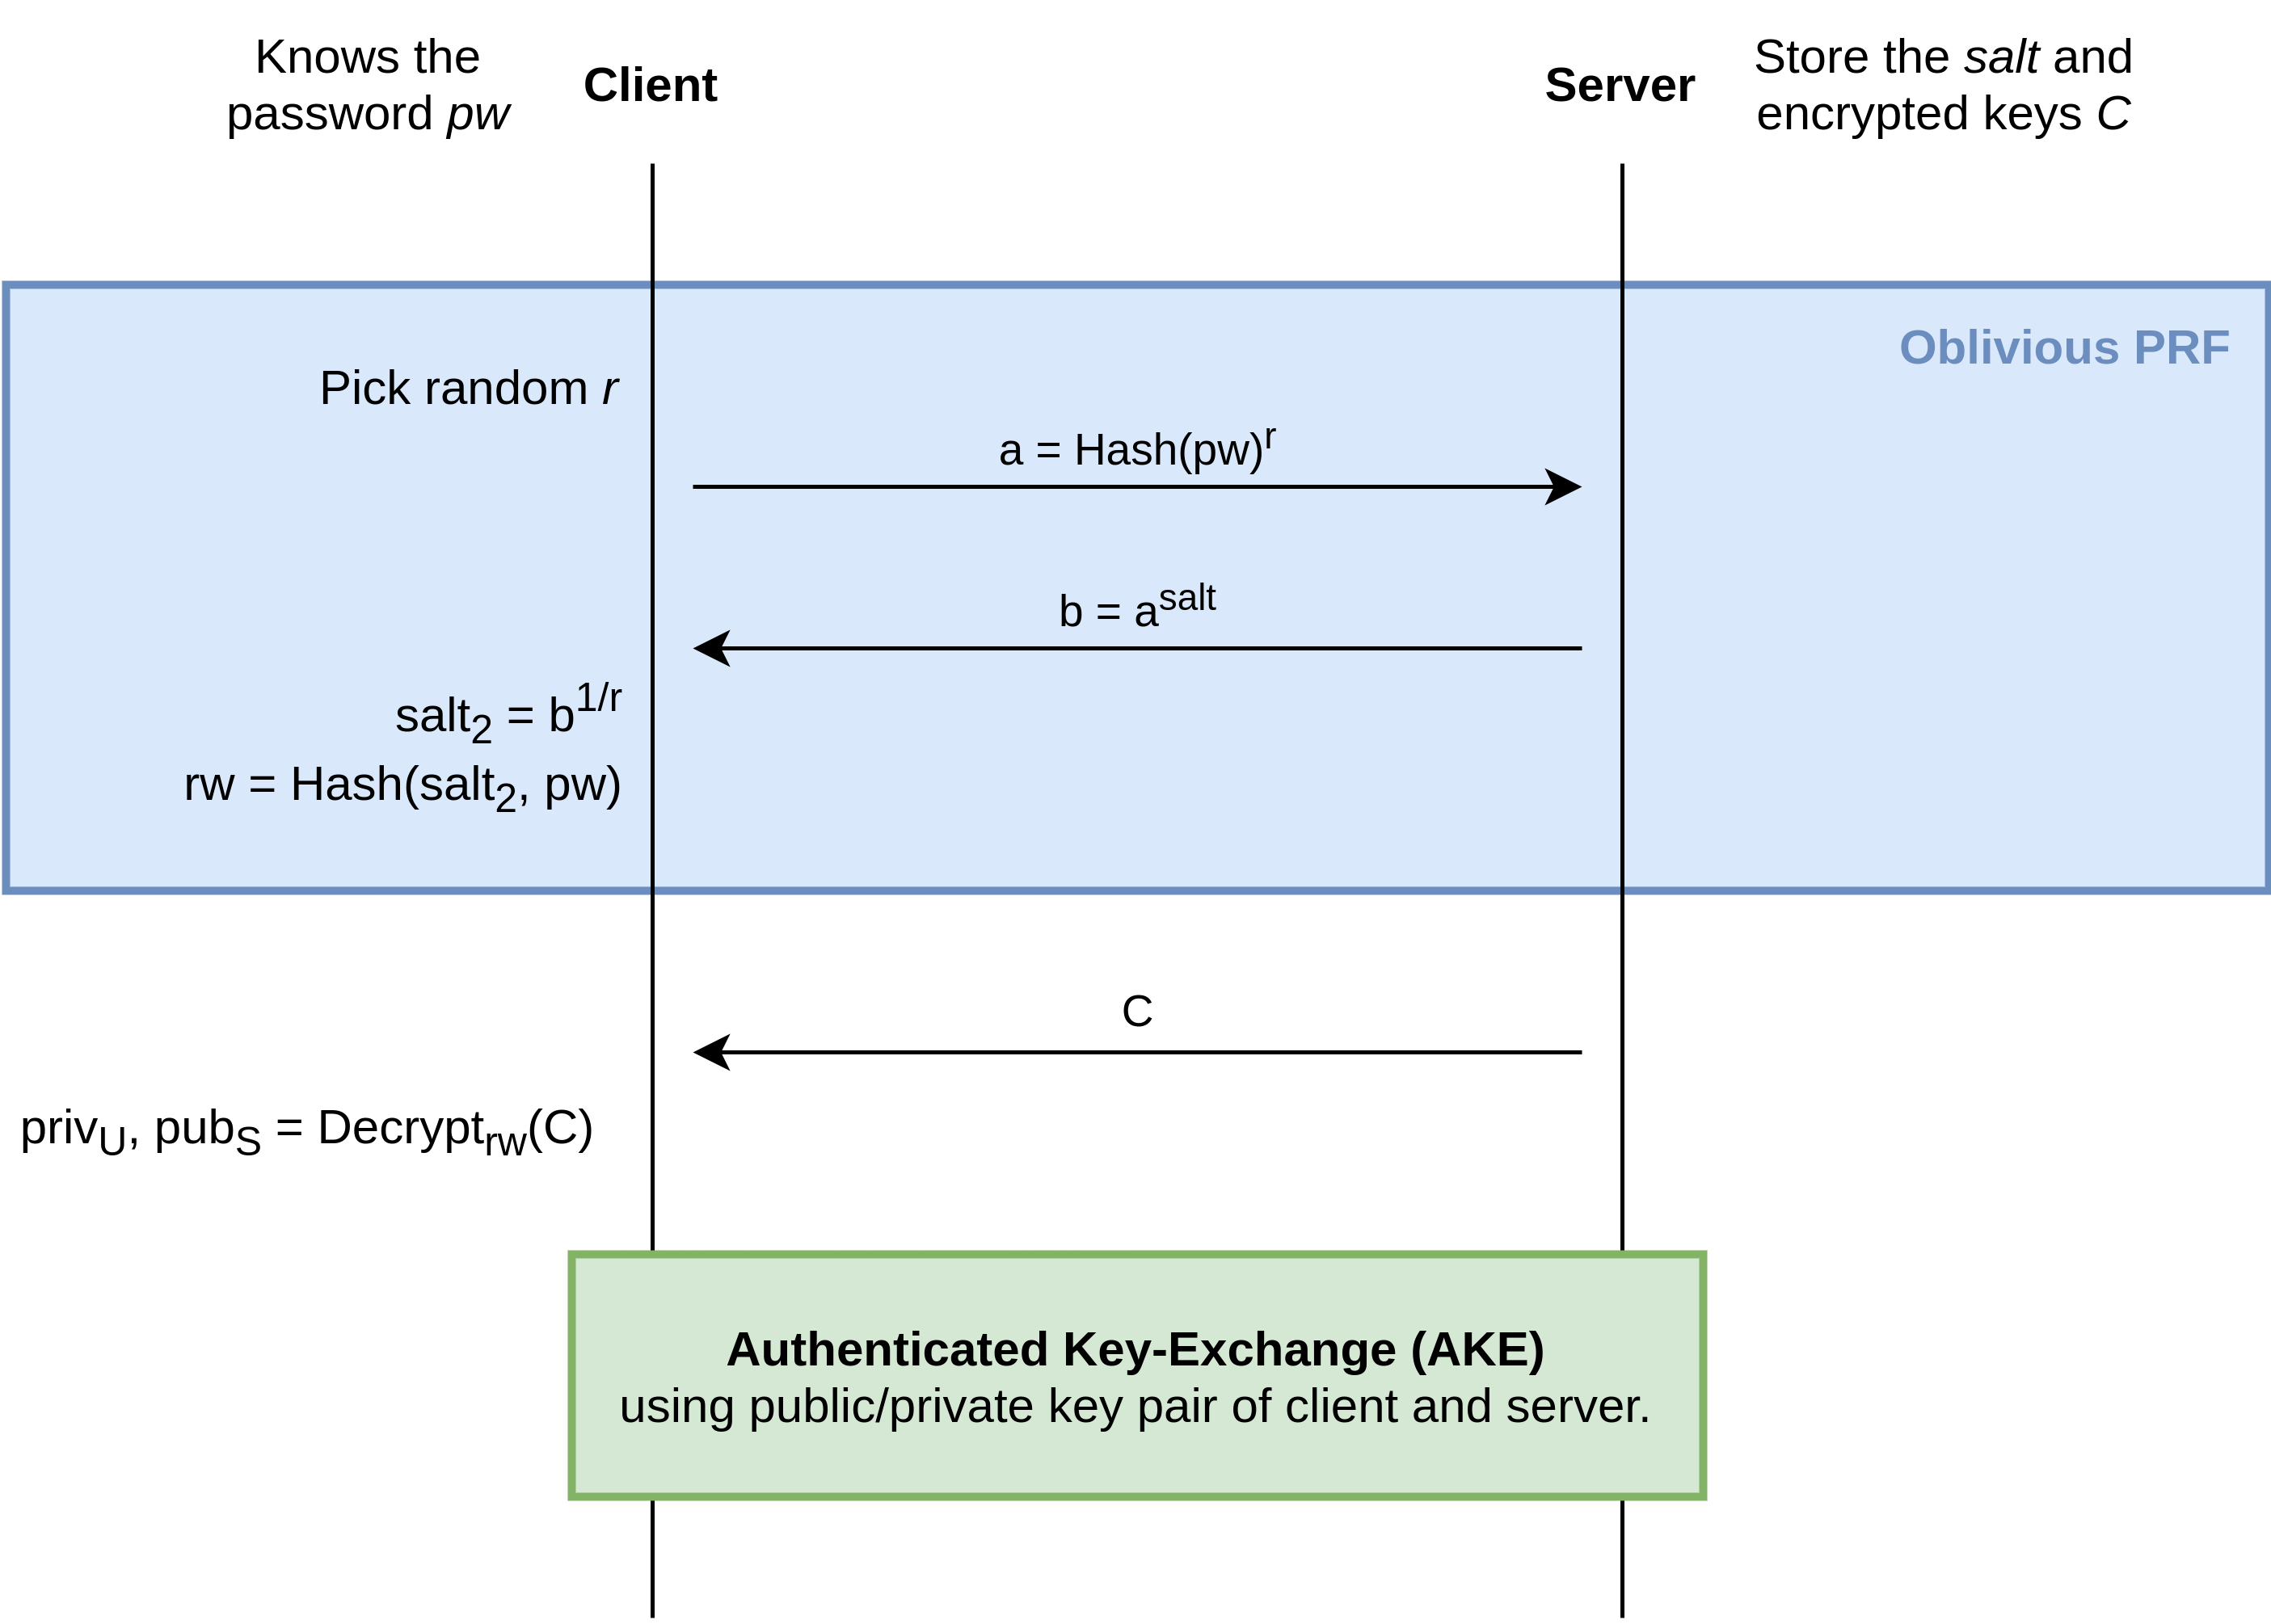
\includegraphics[width=\textwidth-22pt]{OPAQUE.png}}
 \caption{Login process with generic OPAQUE (OPRF-AKE) protocol.}
 \label{fig:OPAQUE_AKE}
\end{figure}
The figure \ref{fig:OPAQUE_AKE} shows the OPAQUE protocol --- built with OPRF and AKE --- during login process.
The steps are the following :

\begin{enumerate}
 \item Generate a random value $r$ to blind the hash of passwords so that the server cannot retrieve the password from the mapping.
 \item Send result to the server.
 \item Server add the salt to the password.
 \item The client calculates the exponent of the inverse of $r$ to de-blind the value. He cannot retrieve salt.
 \item With the secret salt $salt_2$, client compute secret key $sk$.
 \item Server send encrypted keys $C$ to clients. $C$ contains server's public key and client's private key encrypted with $rw$.
 \item If the password entered is correct, client uses $rw$ to decrypt $C$ and retrieve his private key $priv_U$.
 \item With both keys, client and server run an authenticated key exchange for mutual authentication.
\end{enumerate}

\paragraph{\writingFormulationClean{Register.}} \label{sec:opaque_register}
The client registration is the only part of the protocol that requires a secure channel where both parties can authenticate each other.

The protocol is proposed with a server-side registration where the client sends his password through the secure channel. The server generates a salt and computes OPRF function with the client's password and salt. Server also generates two private keys (one for the client and one for the server) and their corresponding public key. He encrypts client's private key and server's public key with OPRF output as a key and store the ciphertext.

This method is not ideal as it requires that the user send its cleartext password to the server making it vulnerable to miss-handling or server-side vulnerabilities discussed in the introduction.

\cite{OPAQUE_Paper} also note that ideally, one wants to implement a client-side registration where the client choose a password and the server choose a secret salt and input them in the OPRF function. The client generates a public/private key pair, and the server do the same. Server sends his public key to the client. Client encrypts his private key and server's public key using OPRF output as a key. He then sends the ciphertext to the server with his public key.
This way, the server never see the cleartext password, the OPRF output and the client's private key. This is a major improvement in terms of security.
However, this also comes with a downside as the server is no longer able to check password rules. This operation needs to be done client side.

\paragraph{\writingFormulationClean{Login.}}
For the login phase, the client enters its password in the OPRF and the server send the ciphertext to the client.
If the password entered is correct, the client can decrypt the ciphertext with OPRF output to obtain his private key and the server's public key.
He then uses these keys to run an authenticated key exchange with the server.
On the other hand, if the password is wrong, the OPRF output is totally different and the ciphertext decryption makes the keys incorrect and the server will refuse it during the key exchange. % TODO confirmation

\paragraph{\writingFormulationClean{Differences with the internet standard draft.}} \label{sec:opaque_paper_vs_draft}
OPAQUE's paper \cite{OPAQUE_Paper} and OPAQUE's internet standard draft \cite{OPAQUE_Standard_Draft} have some differences. The standard draft has evolved in the last 3 years and is now at version 7 (15th iteration).
The draft standard is now much more detailed than before.

One of the major differences in the core protocol design is the encryption of the client's private key.
In the paper, it is specified that the client uses an authenticated encryption scheme to encrypt and decrypt its credentials --- i.e., client's private and public keys and the server's public key. The encryption key is the OPRF output.
In the draft standard, it is rather different.
Firstly, the envelope does not contain the client's keys anymore. It only contains a nonce and an authentication tag. 
The nonce is used --- with a derivation of the OPRF output --- to derive an authentication key, and export key and a seed.
The authentication key is used to verify the envelope,'s authentication tag to ensure that the envelope content has not been modified.
The export key is exposed to the client for application specific usage.
The seed is used to derive the client's key pair.

The envelope is not encrypted at rest anymore. It is only encrypted during transmission between the client and the server with a one-time pad encryption. The rest of the time, the envelope is stored in cleartext on the server.
During registration, the client derives a masking key from the OPRF output and sends it to the server with the envelope. The server stores the envelope and the masking key.
Then, at login, the server generates a masking nonce and derive a one-time pad key using masking keys and masking nonce. He encrypts the envelope and his public key with the one-time pad key and sends the ciphertext with the masking nonce to the client.
The client can compute the masking key with the OPRF output to compute the one-time pad key and decrypt the envelope.


Note that the standard is still in a draft state and is susceptible to be modified.


% ====================================================================================

\subsection{\writingFormulationBrut{KHAPE}}
\paragraph{\writingFormulationBrut{Introduction.}}
OPAQUE security relies entirely on the strength of the OPRF. If OPRF gets broken --- for example by cryptanalysis, quantum attacks or security compromise --- an adversary can compute an offline dictionary attack on the user's password. This is especially critical considering that there are currently no known quantum-safe OPRFs.
KHAPE (for Key-Hiding Asymmetric PakE) \cite{KHAPE_Paper} is a variant to the OPAQUE protocol. Instead of using OPRF as a main tool to archive security, it becomes an optional part of the protocol and KHAPE use two other concepts to archive security: non-committing encryption and key-hiding AKE.

KHAPE is not a Strong aPAKE like OPAQUE. But it can be made a SaPAKE following the aPAKE to SaPAKE compiler from \cite{OPAQUE_Paper} using OPRF.
So OPRF is optional with KHAPE and just allow making it a SaPAKE. In addition, it also allows using OPRF features such as a server-side threshold implementation that does not require any change from the client (see all feature in section \ref{sec:opaque_oprf}). If OPRF fails, KHAPE just loss these functionalities but the rest of the security remain in contrary to OPAQUE.


% ``Two key ideas are: (i) dispense with authentication of the
% credentials4 and instead use a non-committing encryption where decryption of
% a given ciphertext under different keys cannot help identify which key from a
% candidate set was used to produce that ciphertext; and (ii) using a key-hiding
% AKE. The latter refers to AKE protocols that require that no adversary, not even
% active one, can identify the long-term keys used by the peers to an exchange even
% if provided with a list of candidate keys (a notion reminiscent of key anonymity
% for public key encryption [8]).'' \cite{KHAPE_Paper}

\paragraph{Security without OPRF.}
Like OPAQUE, in KHAPE each party has a private/public key pair that is used to compute the key exchange and the client store its private key and server's public key on the server, encrypted by his password.
Without using an OPRF, an adversary could try to retrieve the ciphertext and the server's public key from a valid key exchange between an existing client and the server.
He can then compute an offline dictionary attack using a list of password candidates to decrypt the ciphertext until he finds a match with the server's public key that he recorded sooner.
To avoid these kinds of attacks, KHAPE use two main mechanisms: Non-committing encryption and key-hiding AKE.
\paragraph{Non-committing encryption.} \label{sec:non_committing_encryption}
Non-committing encryption makes it impossible for an adversary to identify the key used to encrypt the ciphertext event with a list of key candidates. This implies that the decryption of the ciphertext under any possible key provide a valid plaintext (i.e., a valid asymmetric key pair that can be used in the key exchange).
\paragraph{Key-hiding AKE.} \label{sec:key_hiding_ake}
The key-hiding feature makes it impossible for an adversary to use the key exchange (output) to identify the correct private/public key decrypted from the ciphertext using a list of password candidates.
Even if provided with a full transcript of a key exchange between a client and a server and a list of key pair candidates --- including the correct key pair --- the adversary has no better chance than random to guess the right key pair that was used.



% \paragraph{\writingNotes{Mains differences with OPAQUE}}
% - KHAPE is computationally more performant than OPAQUE when the OPRF is not used and the performances become similar when OPRF is used.
% - "KHAPE seems more conducive to post-quantum security via post-quantum key-hiding KEMs."
% 
% - KHAPE allow less AKEs (no signature-based protocols such as SIGMA)
% - KHAPE use ``idea cipher model'', OPAQUE use ``random oracle model'' (stronger ?)
% 
% - with OPAQUE the client learns first if an authentication attempt is succeed or not. with KHAPE, the server learns first which make it easier to count failed attempt in case of an online password guessing attack.
% - KHAPE (without OPRF) cost is ~= same cost as KE cost where OPAQUE cost is about the double of KE cost

% Both client and server needs a public/private key pair to compute a AKE. The client encrypt it's credentials (his private key and server's public key) and store it in the server.

%%% How Key-hiding AKE works ?
%%% Ideal cipher ?

\paragraph{\writingFormulationClean{Construction.}}

\begin{figure}[h]
 \centering
 
 \setlength{\fboxsep}{10pt}
 \setlength{\fboxrule}{1pt}
 \fbox{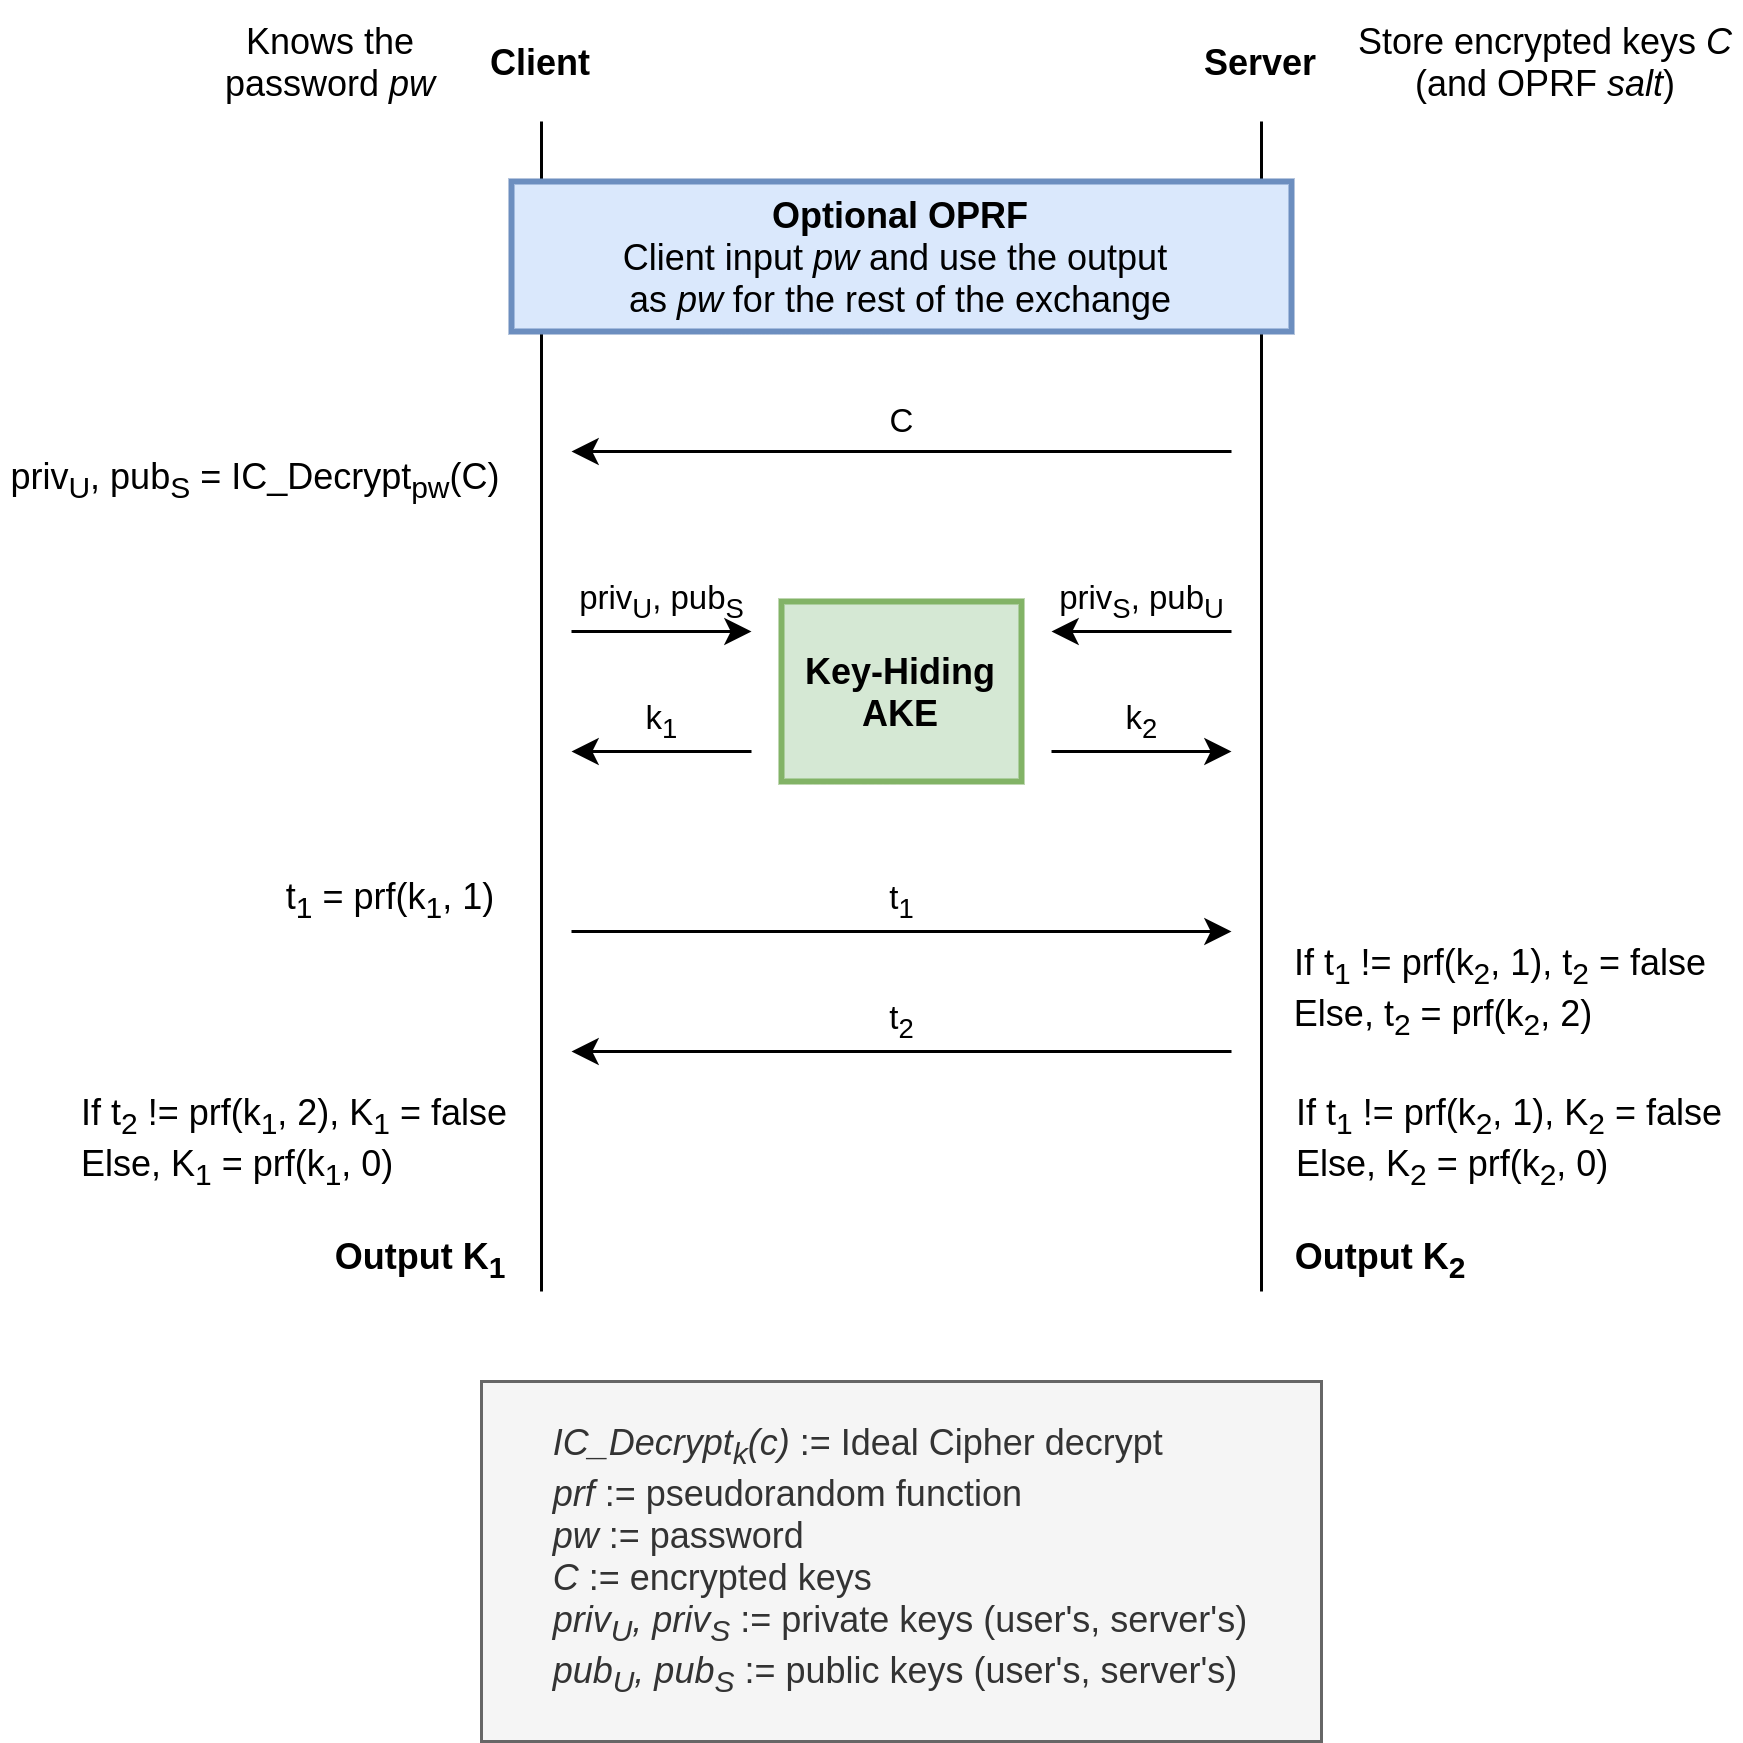
\includegraphics[width=\textwidth-22pt]{KHAPE.png}}
 
 \caption{Login process with generic KHAPE protocol.}
 \label{fig:Generic_KHAPE}
\end{figure}
The figure \ref{fig:Generic_KHAPE} shows the KHAPE protocol during login process.
The steps are the following :
\begin{enumerate}
 \item Optionally, an OPRF can be used to archive Strong aPAKE following the aPAKE to SaPAKE compiler using OPRF from \cite{OPAQUE_Paper}. The OPRF takes the client's password and server's salt as an input. Client uses the output in place of his password for the rest of the protocol.
 \item The server sends the client's encrypted envelope containing the client's private key and server's public key.
 \item The client decrypts the ciphertext using Ideal Cipher encryption schema. He uses his password or OPRF output as a key.
 \item Both parties use the public/private keys to compute a Key-Hiding Authenticated Key-Exchange.
 \item Mutual key-confirmation process initiated by the client.
\end{enumerate}
%%% Login and register steps
\paragraph{\writingFormulationBrut{Login.}}
When the client wants to login, the server sends its encrypted credentials and the client use its password to decrypt the credentials (with or without OPRF depending on the implementation). Then he can use his credentials to compute a Key-Hiding AKE with the server.
Both party finish with a mutual key confirmation initiated by the client.

\paragraph{\writingFormulationBrut{Register.}}
KHAPE has the same problem that is addressed in \ref{sec:opaque_register}.
The protocol proposes a server-side register which is less than ideal because the server can see the client's password and client's private key in cleartext at registration.
Instead, the paper proposes a client-side registration process.

% ====================================================================================

\section{\writingNotes{Comparing main solutions}}
This section compares the main PAKEs on their security guarantees and performances. Details and comments on each criterion can be found on Section \ref{sec:comparison_details}.
 
\subsection{Details} \label{sec:comparison_details}

\paragraph{\writingFormulationClean{1. Server does not process passwords in cleartext.}}
This is the main security property of asymmetric PAKE \cite{aPAKE_Formalized}. Server does not have to store passwords in cleartext which should make it more resilient in case of server compromise. Adversary has to compute an offline attack to retrieve passwords from the compromised server.
\paragraph{\writingFormulationClean{2. Avoid sending cleartext password to the server.}}
Even though it seems similar to criteria 1, it is not. Criterion 1 is about password processing, but this criterion is about password transmission. Transmission and processing of passwords are vulnerable to different attacks vectors.
The server does not receive passwords in cleartext which avoid any miss-handling vulnerabilities such as logging or caching cleartext passwords on the server.
COMMENT: May be required during register depending on the implementation (See Section \ref{sec:opaque_register}).
\paragraph{\writingFormulationClean{3. Secure against pre-computation attacks.}} \label{sec:secure_against_pca}
This is the main security property of Strong aPAKE \cite{OPAQUE_Paper}. The server does not leak any data that could allow an attacker to perform a pre-computation attack (for example SRP send the salt in cleartext in the first message). This attack allows an attacker to compute a table \emph{before} the server even get compromised. Once the attacker succeeds in compromising the server, he can use the precomputed table to retrieve the passwords \emph{instantaneously}. With this protection, an attacker can only perform an offline dictionary attack \emph{after} successfully compromising the server.
This protection is provided by the OPRF (see Section \ref{sec:opaque_oprf}).
% This vulnerability weaken the initial benefit of using an aPAKE \cite{aPAKE_Formalized} and even make password-over-TLS more secure \cite{OPAQUE_Paper} (than aPAKE vulnerable to pre-computation attacks).

\paragraph{\writingFormulationClean{4. Forward secrecy.}}
In key-exchange protocol, Forward Secrecy (also called Full Forward Secrecy or Perfect Forward Secrecy) ensures that upon compromise of any long-term key used to negotiate sessions key, an attacker cannot compromise previous session keys.
In detail key-exchange protocol use long-lived keys to authenticate the user and short-lived keys to encrypt sessions. With Forward Secrecy, an attacker that successfully compromised a long-lived key cannot retrieve any previous session data even if he recorded the previous encrypted transmissions. % TODO cite Duc CAA 05-password ?
COMMENT: For EKE, only DH-EKE provide forward secrecy. ElGamal-EKE and RSA-EKE does not.
\paragraph{\writingFormulationClean{5. Mutual authentication.}}
Mutual authentication explicit that users must be authenticated to the server but also that the server must authenticate itself to the user to avoid that an adversary impersonates the server to maliciously communicate with the client.
\paragraph{\writingFormulationBrut{6. PKI-free.}} % TODO rename to: Doesn't require transmission over a secure channel
The transmissions between client and server does not require to be secured with Public Key Infrastructure (PKI). This is a big improvement over classical authentication method (password-over-TLS) considering the occurrence of PKI failures nowadays. % "PKI failures include stealing of server private keys, software that does not verify certificates correctly, users that accept invalid or suspicious certificates, certificates issued by rogue CAs, servers that share their TLS keys with others e.g., CDN providers or security monitoring software, information (including passwords) that traverses networks in plaintext form after TLS termination; and more."
\paragraph{\writingFormulationClean{7. User-side password hardening.}} \label{sec:password_hardening_comparison}
Users can use password hardening technique to increase the cost of an offline attack if the server gets compromised. This is done by using resource-heavy functions such as Scrypt \cite{Scrypt_Paper} or Argon2 \cite{Argon2_Paper} instead of computing a simple and efficient hash. These functions allow to drastically slows down hashing process and so making offline attacks and online guessing attack much slower.
COMMENT: For EKE, it could be possible to compute a KDF function on the password before using it as a symmetrical key but this is closer to Augmented EKE \cite{AEKE_Paper} where the password is hashed client side and the server store the hash results.
For SRP, the client-side operation $x = H(salt||pwd)$ can be modified to use a resource-heavy hashing function \cite{SRP_1Password_blog}.
\paragraph{\writingFormulationBrut{8. Built-in mechanism to store client's secrets on the server.}}
%OPAQUE "has a built-in facility for password-based storage-and-retrieval of secrets and credentials"
%~~New protocol such as OPAQUE and KHAPE use client-side decryption of server-stored ciphertext to retrieve the key. This allows running exchange in an unsecured channel because...
Securely store client's sensitive data such as secrets or credentials in the server without the server being able to read it. With OPAQUE and KHAPE, the user credentials (private/public keys) are encrypted with the password or OPRF output and then stored in the server. Additional secrets specific to the application could be added to this encrypted envelope and stored on the server.
\paragraph{\writingFormulationBrut{9. Server threshold implementation.}}
%OPAQUE "accommodates a user-transparent server-side threshold implementation."
Require the interaction with $n$ servers to authenticate. This means that $n$ server has to be compromised in order for an adversary to compute an offline dictionary attack on the password. This scenario can be useful in the case of a highly sensitive application.
OPRF transparently provides this functionality where each server adds its independent secret salt to the blinded password hash before sending it back to the client.
\paragraph{\writingFormulationClean{10. Resistant upon Oblivious PRF compromise.}}
This criterion is a bit arbitrary because only the two recent PAKE uses an OPRF but it is still an important criterion because it is the main difference of security guarantees between OPAQUE and KHAPE.
If OPRF breaks for example by cryptanalysis, security compromise or even quantum attacks, the consequences could be disastrous depending on the way it is used. This is especially important because there is ``currently no known efficient OPRFs considered to be quantum safe'' \cite{KHAPE_Paper}.
OPAQUE use OPRF as a main tool to builds Strong aPAKE. If OPRF breaks, the client's password is vulnerable to an offline dictionary attack.
KHAPE has a weaker reliance on OPRF. It is optional and only used to archive Strong aPAKE. If OPRF breaks, KHAPE only fall back to a non-strong aPAKE (making it vulnerable to pre-computation attacks). 
This makes KHAPE more resistant to OPRF compromise than OPAQUE. 

\paragraph{\writingNotes{11. Standardization status.}}
The standardization status is a good indicator to the maturity and adoption of a construction.
% As it show that the construction is discussed. Generally, standard are far more precise 
% Standards allow a better inter operability and easier implementation.
\paragraph{\writingNotes{12. Security proof.}}
%OPAQUE "security proof in a very strong model"
COMMENT: EKE only provide informal security analysis \cite{EKE_Informal_Security_Analysis}
SRP provide no valuable security proof \cite{CAA, SRP_Green_blog}. It only proves that it can stand up to passive attacks, which is not enough for an authentication protocol. A proof against active attacks would be welcomed for such a widely used protocol.
\paragraph{\writingNotes{13. Easily adaptable to elliptic curves.}} \label{sec:ecc_comparison}
Elliptic curve cryptography allows to greatly reduce the size of asymmetric key.
This is crucial in terms of performance because key size recommendations are always growing to ensure security and asymmetric keys are getting giant and difficult to manage --- in particular for keys that require long-term protection (up to 50 years). For example, for such a long-term protection, the discrete logarithm group is recommended to be 15,360 bits according to ECRYPT-CSA \cite{ECRYPT_Keylength}.
In comparison, with elliptic curves, only 512 bits are recommended to archive similar security levels.
COMMENT: 
In SRP, $\mathbb{Z}_p$ is used as a field, not a group. Therefore, SRP cannot be easily adapted to elliptic curves \cite{CAA}. % TODO voir SRP_Green_blog
% TODO ``SRP requires a ring as it mixes addition and multiplication operations, and thus does not work over plain elliptic curves''

For DH-EKE, it is required that the content that will be encrypted --- namely $A$ and $B$ --- must be indistinguishable from random data. 
This requirement makes it impossible to implement it on elliptic curves \cite{EKE_ECC}. %also source : https://tools.ietf.org/id/draft-ietf-kitten-krb-spake-preauth-00.html#rfc.section.1.2
% An implementation on elliptic curve wouldn't satisfy this requirement.

% ``One of the most well-known variant of EKE is Diffie-Hellman EKE
% (DH-EKE) which is merely a DH key exchange where at least one message
% exchanged under DH is encrypted via the password. Bellare et al. introduced in [3] a formal security model to grasp the specificity of passwordbased key exchange. This model was used later in [9, 10] to establish the
% security of DH-EKE under ideal assumptions (namely the ideal cipher
% model and the Random Oracle Model, ROM). However ideal cipher model
% is not easily applicable to elliptic curves and thus in its classical version,
% DH-EKE is not well adapted to elliptic curves. A naive application of the
% encryption step of DH-EKE to elliptic curves points would lead to an insecure scheme. Indeed, due to the redundancy in a point representation,
% partition attacks [15] are made possible to distinguish possible passwords
% from impossible ones and the security against offline dictionary attacks
% does not hold (the main idea is that a decryption with a bad password of
% an encrypted point would most probably not be a point over the elliptic
% curve). In [8], a modification of the scheme is suggested by using either
% a point of the curve or a point over its twist. Although, this enables to
% withstand the security issue, the scheme is not proved in the model of [3]
% and becomes much less simple than DH-EKE.'' \cite{EKE_ECC}
% ``Finally, in both cases, DH-EKE and SPEKE do not hide the curve
% parameters as they can easily be deduced from 2 eavesdropped points.'' \cite{EKE_ECC}

\paragraph{14. Number of messages.}
more messages means ``increasing latency and loads on the network''

\paragraph{15. Number of exponentiations.}

\paragraph{16. Computational cost compared to a KE (see \cite{KHAPE_Paper} presentation).}

\paragraph{17. Communication size.}

\paragraph{18. Server-side storage size.}

\paragraph{19. Patented.}

\paragraph{20. Year published.}

\paragraph{21. Got broken.}


\subsection{Table}
For value where there is a ``*'', please refer to the appropriate comment in Section \ref{sec:comparison_details} for precision.
\begin{center}
   \begin{tabular}{ | c | p{5cm} || p{2cm} | p{2cm} | p{2cm} | p{2cm} | }
     \hline
     \textbf{\#} & \textbf{Criteria} & \textbf{EKE} & \textbf{SRP} & \textbf{OPAQUE} & \textbf{KHAPE} \\ \hline
     
     % Content :
     
     % Qualities (security guarantees)
     
     1 & Server does not process passwords in cleartext & No & Yes & Yes & Yes \\ \hline
     2 & Avoid sending cleartext password to the server & No & Yes & Yes* & Yes* \\ \hline
     
     3 & Secure against pre-computation attacks & - (no hash) & No & Yes & Yes, if using OPRF \\ \hline
%      3 & Server doesn't send salt in cleartext & - (no salt) & x & Yes & Yes (OPRF) (without OPRF there is no salt) \\ \hline
     4 & Forward secrecy & Yes* & Yes & Yes & Yes \\ \hline
     5 & Mutual authentication & Yes & Yes & Yes & Yes \\ \hline
     6 & PKI-free & Yes, except during register & Yes, except during register & Yes, except during register & Yes, except during register \\ \hline
     7 & User-side password hardening & No* & Yes* & Yes & Yes, if using OPRF \\ \hline
     8 & Built-in mechanism to store client's secrets on the server & No & No & Yes & Yes \\ \hline
     9 & Server threshold implementation & No & No & Yes, user-transparent & Yes, if using OPRF \\ \hline
     10 & Resistant upon Oblivious PRF compromise & - (no OPRF) & - (no OPRF) & No, entire security is compromised & Fall back to non-strong aPAKE \\ \hline
     11 & Standardization status & RFC for EAP-EKE \cite{EAP_EKE_RFC} & 3 RFC \cite{SRP_RFC_1, SRP_RFC_2, SRP_RFC_3}, 1 ISO \cite{SRP_ISO}, 1 IEEE \cite{SRP_IEEE} & Internet standard draft \cite{OPAQUE_Standard_Draft} & CRYPTO 2021 Paper \cite{KHAPE_Paper} \\ \hline
     12 & Security proof & No* & No valuable security proof & Yes, in the random oracle model & Yes, in the ideal cipher model \\ \hline
     
     \end{tabular}
 \end{center}
 
\begin{center}
   \begin{tabular}{ | c | p{5cm} || p{2cm} | p{2cm} | p{2cm} | p{2cm} | }
     \hline
     \textbf{\#} & \textbf{Criteria} & \textbf{EKE} & \textbf{SRP} & \textbf{OPAQUE} & \textbf{KHAPE} \\ \hline
     % Performances
     
     13 & Easily adaptable to elliptic curves & No* & No* & Yes & Yes \\ \hline
     14 & Number of messages & 4 ? & 4 ? & 3 & 4 (3 if client initiate) \\ \hline
     15 & Number of exponentiations & 4 ? & 4 ? & 3 or 4 ? & 2 + 1 hash-to-curve \\ \hline
     16 & Computational cost compared to a KE (see \cite{KHAPE_Paper} presentation) & 1x & TBD & 2x & 1x without OPRF, 2x with OPRF \\ \hline
     17 & Communication size & TBD & TBD & TBD & TBD \\ \hline
     18 & Server-side storage size & TBD & TBD & TBD & TBD \\ \hline
     
     19 & Patented & Yes, expired in 2011 & No & No & No \\ \hline
     20 & Year published & 1992 & 1998 & 2018 & 2021 \\ \hline
     21 & Got broken & Some versions got broken & Yes and patched \cite{CAA} & No & No \\ \hline
     \end{tabular}
 \end{center}


\end{document}
